\documentclass[12pt]{article}

\usepackage[utf8]{inputenc}
\usepackage[T1]{fontenc}
\usepackage{geometry}
\usepackage{graphicx} %figures
\usepackage{subfig} %subfigures
\usepackage{gensymb} %degree sign
\usepackage{amsmath} %math stuff
\usepackage{bm} %bold stuff
\usepackage[]{algorithm2e} %algorithms
\geometry{a4paper}

\title{Part 15: GPYtorch and Custom Kernels}

\begin{document}
\date{March 8, 2021}
\maketitle

This post will be focused on using \emph{GPYtorch} tools to make a custom kernel matrix for use in Gaussian processes. We are using this tool because there is an ecosystem of python \emph{torch} tools were hyperparameter optimization, constraints, priors, and integration are built into the code, providing easy access to tools much more powerful than what I can code in a week.

\section{GP Regression using \emph{GPYtorch}}

We start by modeling $y=sin(2\pi) + \epsilon$ using a GP with constant $\mu(x)$ and $\Sigma(x,x')=\sigma_f^2 \times \Sigma_{RBF}(x,x',\lambda)$, which is the common GP with radial basis function covariance and scaling parameter.  Using \emph{GPYtorch} we use a standard Gaussian likelihood (which has been shown in other posts) to train the model using autograd functions to construct gradients for use in ADAM optimizer of hyperparameters. We have already gone over stochastic gradient descent and other optimizers for random functions so I won't go into the details (we may do a post on how \emph{GPYtorch} does this in the future). This is also the simplest GP model we usually consider because it only has one length-scale parameter, one output-scale parameter, and one noise parameter. With some random data $N$ and dimension $p=1$ we get nice regression.

\begin{figure}[h]
\centering
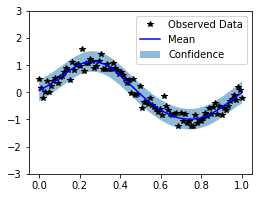
\includegraphics[width=0.6\textwidth]{Post_15_regulargp}
\caption{Sinusoidal Regression using \emph{GPYtorch} GP}
\end{figure}

\section{Custom Hyperparameters}

If we want to implement custom hyperparameters that needs to be done in our \emph{CustomKernel} class. I have coded a generic \emph{lengthscale} and \emph{outputscale} attached to the \emph{self} provided in python, and shared it in the \emph{forward} subfunction. This subfunction does the heavy lifting in the code using \emph{numpy} and is re-converted to tensors. For the interested, I have added (i) a generic RBF kernel, (ii) a multi-fidelity kernel, and (iii) a linear kernel.

\section{Custom Kernels}

The interesting custom kernel implemented here is a multi-fidelity kernel. See previous posts for multi-fidelity Bayesian optimization and modeling. The problem here will just be noiseless $Y=X$ with regularly spaced input points. For the 'true' fidelity we'll use $N=5$ points $[0.5,1]$ and for the lower fidelity we'll use $N=5$ points $[0,0.5]$. If it works, the multi-fidelity model will be able to use the lower fidelity points to better predict the line, whereas the normal GP, not having access to those points, cannot. From Figure 2 we see that this is the case. 

\begin{figure}[h]
\centering
\subfloat[][Fidelity 0]{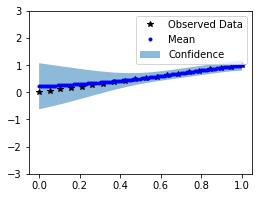
\includegraphics[width=0.3\textwidth]{Post_15_0}}
\subfloat[][Fidelity 1]{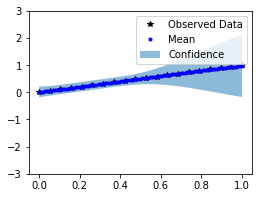
\includegraphics[width=0.3\textwidth]{Post_15_1}}
\subfloat[][Regular GP]{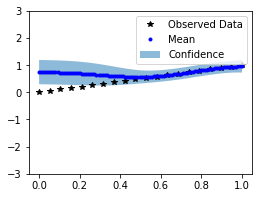
\includegraphics[width=0.3\textwidth]{Post_15_gp}}
\caption{Custom Kernel Experiments | custom multi-fidelity kernel using $N=10$ data points vs regular kernel using $N=5$ data points}
\end{figure}

\vspace{5mm}

That's pretty much what I wanted to talk about here. We didn't learn about any new cool models only some code stuff so the juicy details are in the python code. Next week we'll do more fun modeling stuff with GPs using linear basis functions.

\end{document}